\chapter{Návrh riešenia}\label{chap:proposal}

Cieľom práce je detegovať reklamné plochy pri cestách z video nahrávky a odhadnúť ich významnosť. Kapitola je venovaná návrhu, podľa ktorého sme vypracovali riešenie.  

% Významnosť reklamy priamo súvisí s tým, na aký dlhý čas vodič stratí pozornosť jej sledovaním. Postup, ktorý sme zvolili, je na obrázku \ref{plan} a bližšie opísaný v kapitole. 

% Aby sme z videa vedeli detegovať reklamy, potrebovali sme natrénovať neurónovú sieť. Na tréning sme museli nájsť dostatočne veľký dataset reklám. Pre nás bolo dôležité detegovať trajektóriu reklamy, preto sme okrem detektora potrebovali algoritmus, ktorý identifikuje tú istú reklamu vo viacerých snímkach.

\section{Detekcia reklám}

Na detekciu reklám sme použili konvolučnú neurónovú sieť. Navrhli sme sieť YOLOv8 \cite{yolov8}, ktorá bola predstavená na začiatku tohto roka so sľubným vylepšením oproti predchádzajúcim verziám. Na trénovanie sme použili dataset Mapillary Vistas, ktorý bol uvedený v podobných prácach. Obsahuje 25000 obrázkov s desiatkami tried, vrátane triedy bilbord a banner.

% \begin{figure}[ht]
%     \centering
%     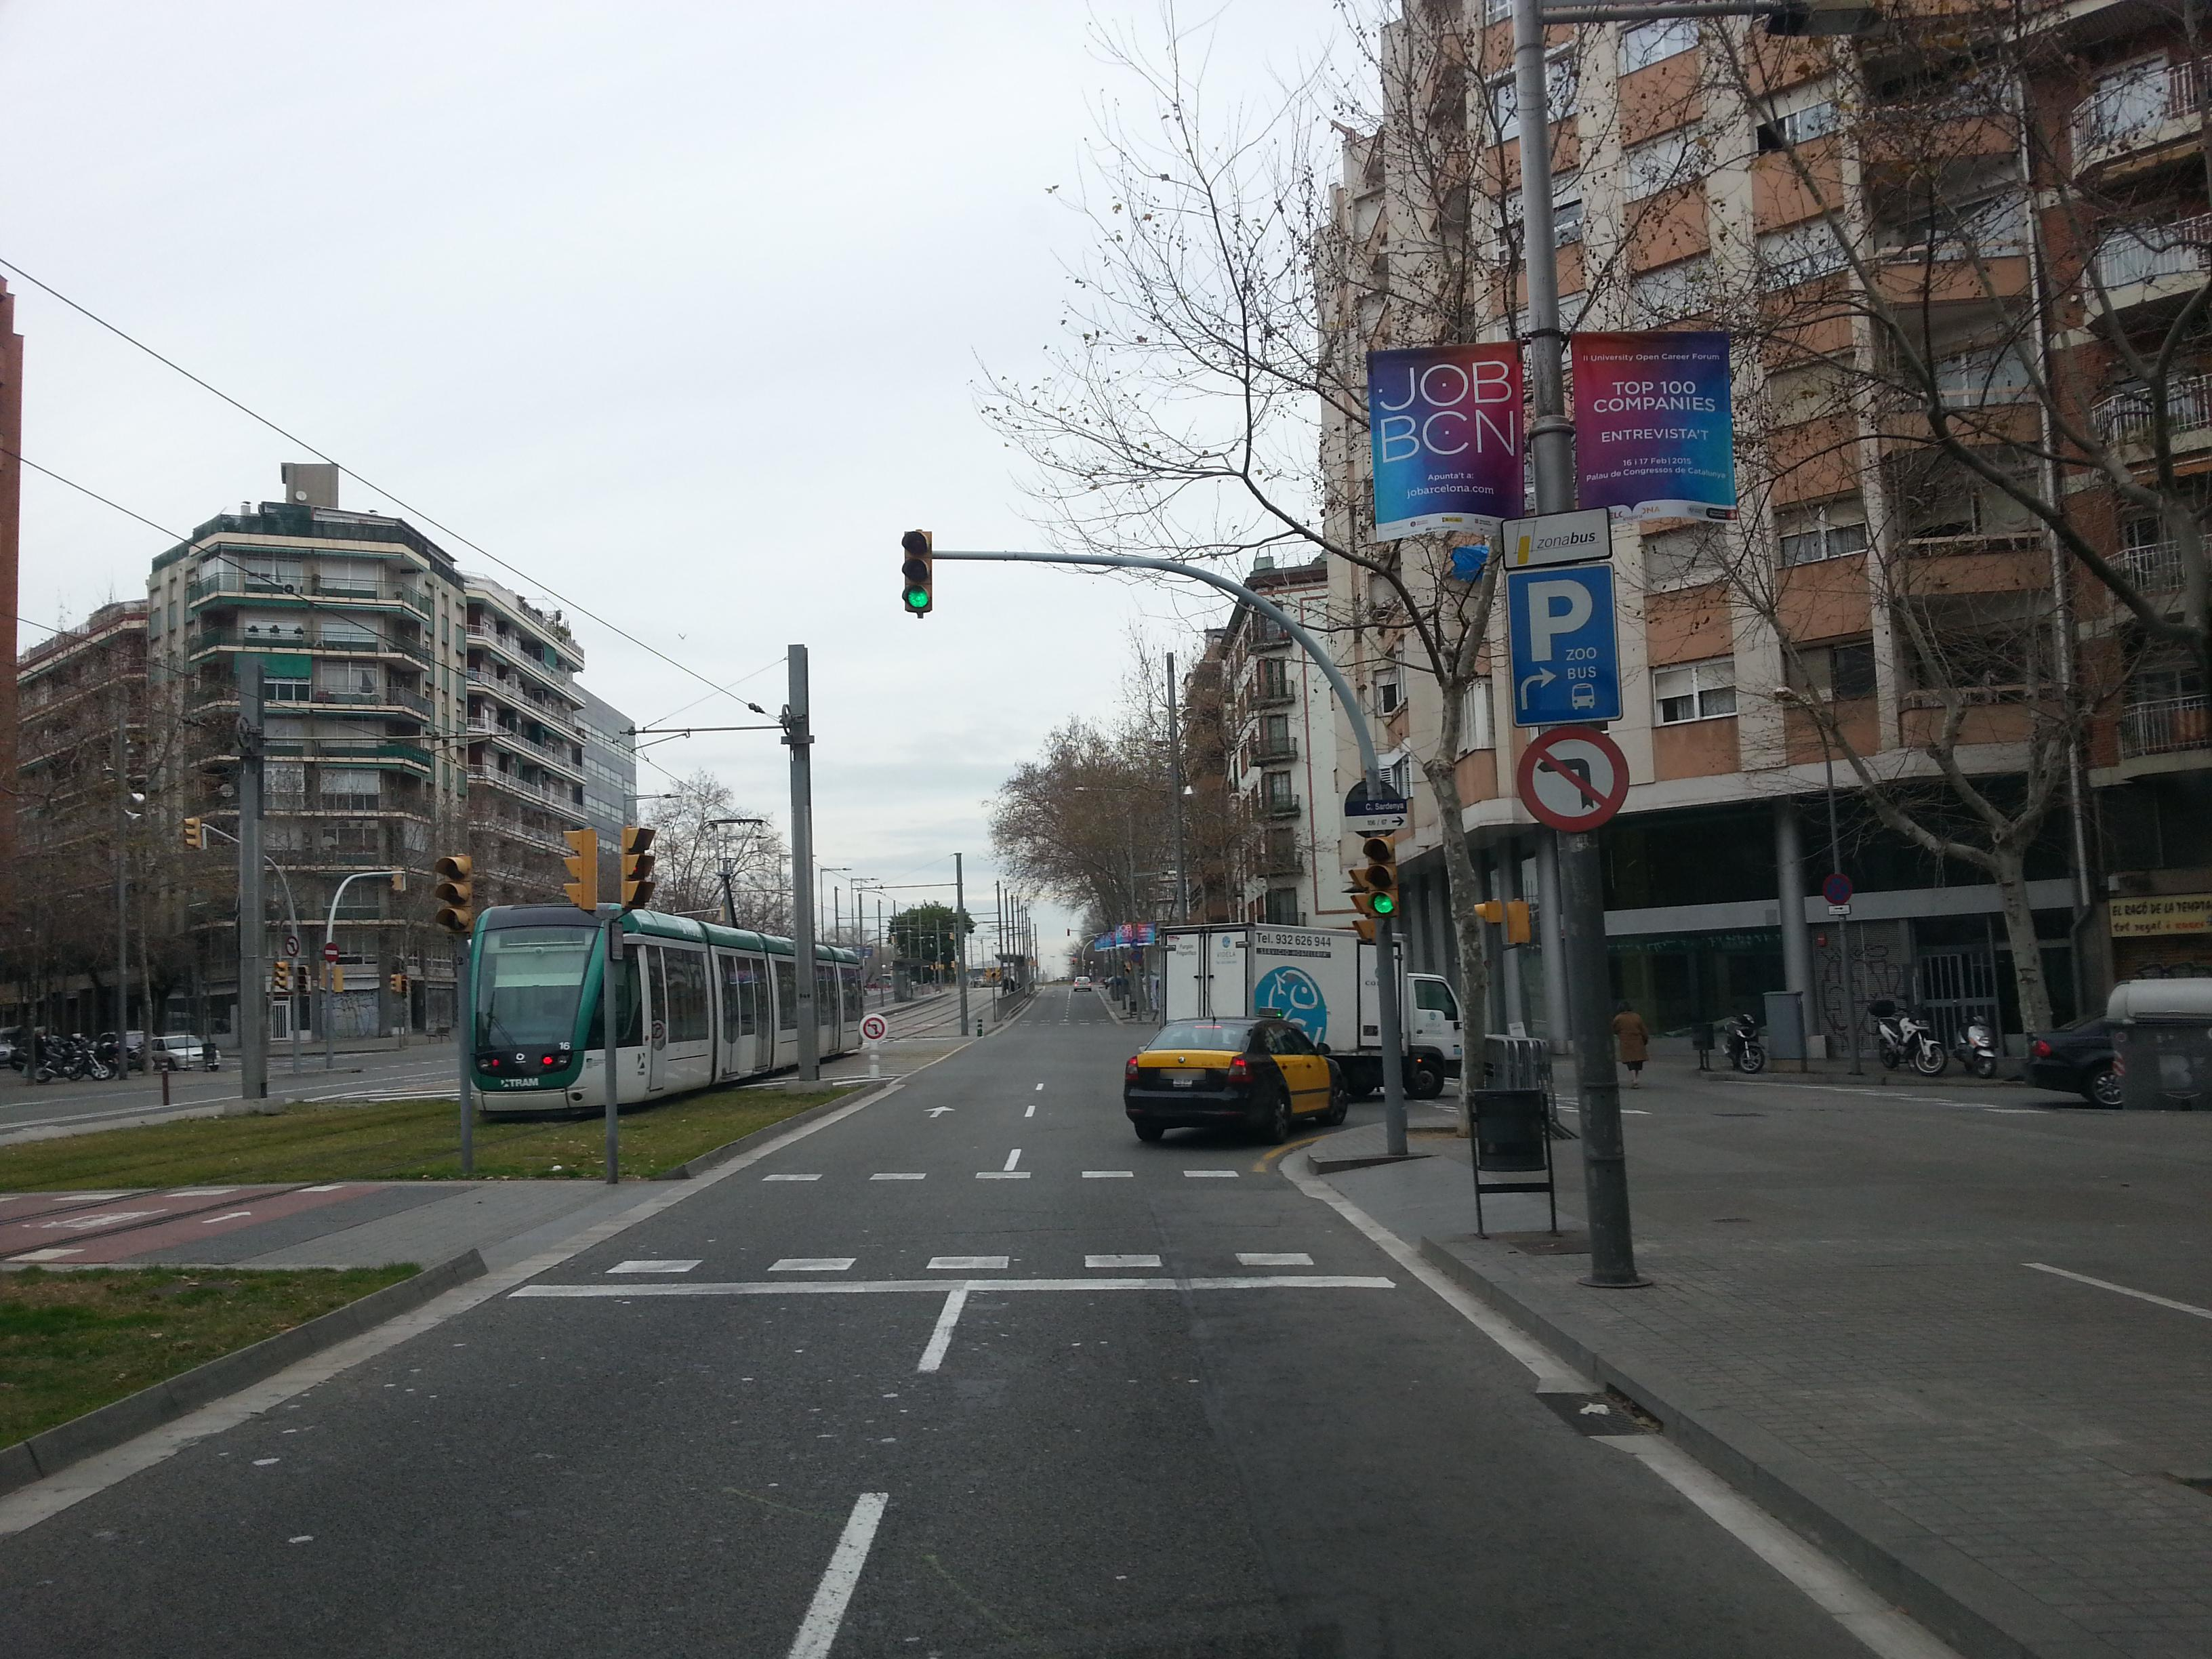
\includegraphics[width=1\textwidth]{images/02/mapillar.jpg}
%     \caption{Ukážkový obrázok z datasetu Mapillary Vistas.}
%     \label{img:dataset}
% \end{figure}

% Obrázky sú zachytené z auta, v hustejšej premávke vo vnútri mesta, kde sa nachádza veľa budov, chodníkov a dopravných značení. Nevýhodou môže byť vysoké rozlíšenie, na ktorom sú označené aj veľmi malé objekty.

\subsubsection{Sledovanie reklám}

% V konečnom prípade nás zaujímali reklamy nachádzajúce sa vo videu, preto sme potrebovali zabezpečiť ich sledovanie. Detektor spracuje video samostatne po jednej snímke. Pre detekciu reklamy vráti len jej lokalizáciu. Algoritmus na sledovanie objektov pre detekciu priradí referenciu na základe asociácie s detekciami na predchádzajúcich snímkach. Ak sa zdá, že podobný objekt už bol na predošlých snímkach, tak mu priradí rovnakú referenciu. Ak medzi predošlými detekciami nenašiel podobný objekt, tak mu priradí novú referenciu.

% Medzi popredné metódy na sledovanie objektov patrí OC-SORT \cite{ocsort}, Deep OC-SORT \cite{deepsort}, StrongSORT \cite{strongsort}, BoTSORT \cite{TODO}, ByteTrack \cite{bytetrack} a mnohé iné. Navrhli sme vyskúšať a porovnať všetkých päť uvedených metód sme vyskúšali a porovnali medzi sebou. Každá metóda je variáciou metódy Simple Online and Realtime Tracking (SORT), ktorá na sledovanie používa Kalmanov filter a Hungarian algoritmus \cite{sort}.

Detektor vyhodnocuje video po jednej snímke a každá detekcia predstavuje samostatnú reklamu. Pre nás bolo dôležité detegovať trajektóriu reklamy, preto sme okrem detektora potrebovali algoritmus, ktorý identifikuje tú istú reklamu vo viacerých snímkach. Navrhli sme vyskúšať viacero sledovacích metód a porovnať ich medzi sebou.

\section{Príprava dát}

Aby sme vedeli odhadnúť významosť reklamy, potrebovali sme mať databázu reklám s priradením významnosti, podľa ktorej by sme natrénovali klasifikátor. Keďže sme takú databázu nenašli, museli sme vytvoriť vlastnú. Pripravili sme experimentálne meranie, od ktorého sme očakávali dostatočnú kvalitu a kvantitu dát pre ďalší proces.

Na zber dát sme mali možnosť použiť eyetracker Tobii Glasses 3, ktorý je k dispozícií na našej fakulte. Eyetracker je zariadenie, ktoré dokáže snímať kam sa človek pozerá a súčasne nahrávať video. 

% Kamera disponuje širokým záberom s rozlíšením 1920x1080. Na sledovanie pohybu šošoviek sú pripravené štyri kamery a ďalších šestnásť osvetľovačov. Všetko je integrované priamo v sklách okuliarov, pričom by nemali nijakým spôsobom brániť vo výhľade. Okrem toho sú sklá jemne zatienené, pretože sú veľmi citlivé na priame osvetlenie.

\begin{figure}[ht]
    \centering
    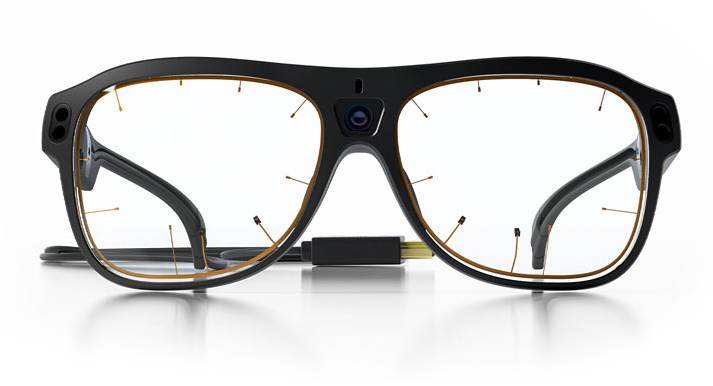
\includegraphics[width=0.5\textwidth]{images/02/glasses.jpg}
    \caption{Eyetracker, model Tobii Glasses 3 \cite{tobii}.}
    \label{img:tobii}
\end{figure}

% Potrebovali sme vytvoriť viacero záznamov jednej trasy, ktorú prejdu viacerý vodiči. 

Aby bolo meranie čo najviac konzistentné, bolo dôležité zabezpečiť rovnaké podmienky pre každého účastníka merania. Na základe prečítaných prác, % ktoré robili podobný zber dát, 
sme vedeli, že pohlavie neovplyvňuje meranie, preto nezáležalo na pomere pohlavia medzi účastníkmi. Naopak, to čo meranie ovplyvňuje je vek a skúsenosť so šoférovaním. Dôležitou podmienkou bola jazda v približne rovnakom počasí a hustotou premávky. 

Sledovaním reklám v našom okolí, sme nakoniec zvolili okružnú jazdu, ktorá je zobrazená na obrázku \ref{img:road}. Odhadovali sme, že na zvolenej trase, ktorá trvá približne 24 minút, sa môže vyskytovať približne 150 reklamných plôch. Trasa bola zvolená kvôli rôznorodosti reklám a jej blízkosti od fakulty.
\\
\begin{figure}[ht]
    \centering
    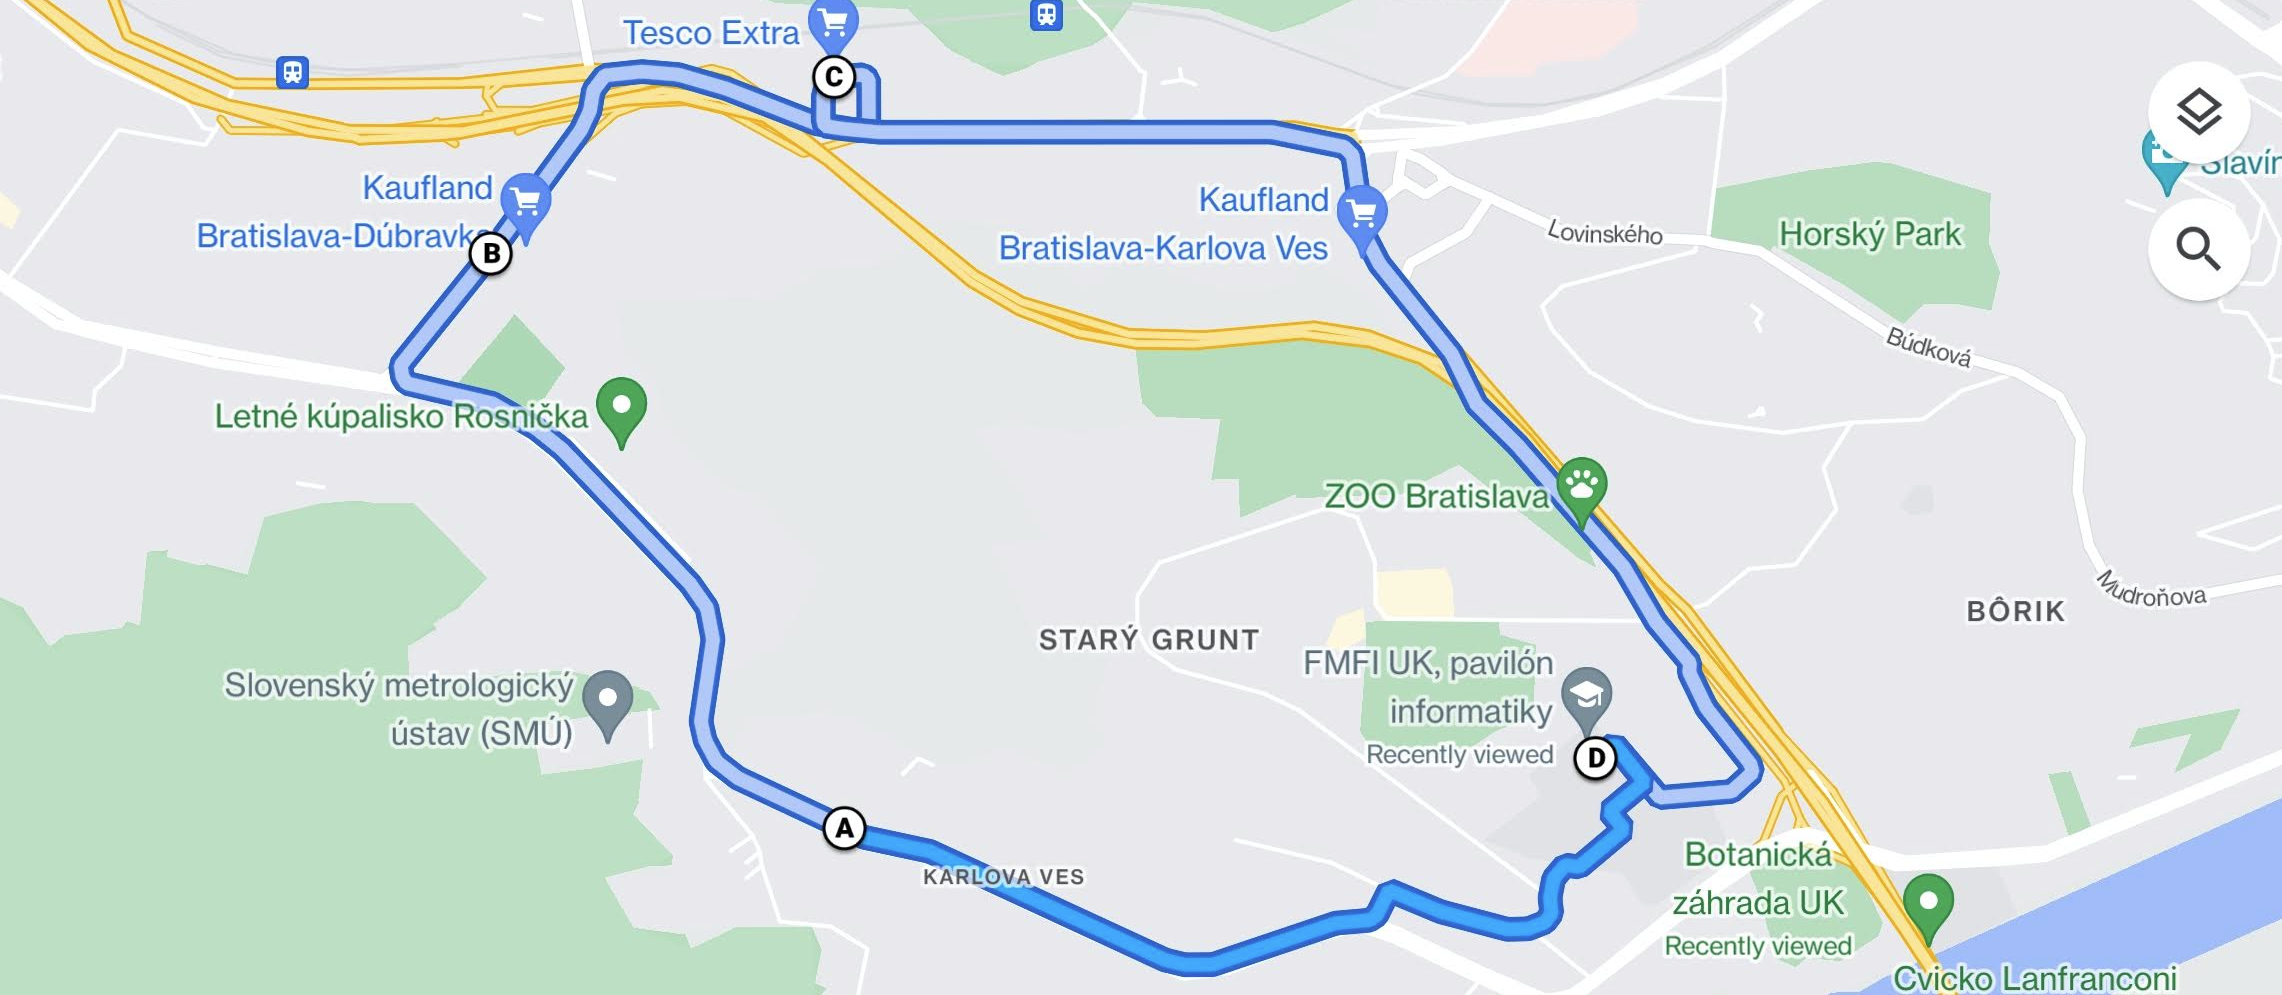
\includegraphics[width=1\textwidth]{images/02/map.png}
    \caption{Fixná trasa zvolená pre experimentálne meranie.}
    \label{img:road}
\end{figure}

% DeepSORT je rozšírením pre SORT, ktorý integruje informácie o vzhľade získané z predtrénovaného modelu. Výsledkom je lepšie priradenie správnej identity čo zároveň redukuje počet vytvorených identít \cite{deepsort}. ByteTrack sa zameriava na asociáciu údajov a navrhuje novú metódu Byte, ktorá sleduje priradenie s porovnávaním každého objektu, ktorý bol doposiaľ zaznamenaný \cite{bytetrack}. OC-SORT je metóda, ktorá používa pozorovanie objektov na výpočet virtuálnej trajektórie počas prekrytia objektu, aby sa zmiernilo hromadenie chýb Kalmanovho filtra, ktoré vzniká počas oklúzie \cite{ocsort}. StrongSORT je varianta, ktorá pridáva pohybový model založený na optickom toku na zlepšenie výkonu sledovania pričom sa snaží kombinovať výhody z metódy Deep SORT a ByteTrack \cite{strongsort}. Každý model má sadu parametrov, ktoré sme jemne upravovali a sledovali zmenu vo výsledkoch. https://www.tasq.ai/blog/object-tracking/

\section{Významnosť reklám}

Spoliehali sme, že sledovanie dosiahne dostatočne dobrú úroveň na to, aby sme spolu s nameranými pohľadmi vodiča vedeli pomenovali významnosť jednotlivých reklám a tým vytvorili malú databázu reklamných plôch. 

% Pre každú snímku, na ktorej bola nájdená reklama sme porovnali prienik so získanou súradnicou miesta, kam sa vodič pozeral v danom okamihu pozeral. Pre každú reklamu sme tak získali informáciu o počte snímok, na ktorých bol prienik s pohľadom vodiča. Počet snímok sme vynásobili dĺžkou trvania jednej snímky, čím sme získali časový údaj fixácie. Podľa dĺžky fixácie sme vyhodnotili významnosť reklamy pre každého vodiča samostatne a následne vypočítali priemer. 

Významosť reklamy sme plánovali rozdeliť do štyroch kategórií podľa priemernej dĺžky sledovanosti: 

\begin{itemize}
  \item slabá: 0ms
  \item nízka: 1 - 249ms
  \item stredná: 250 - 499ms
  \item vysoká: 500ms a viac 
\end{itemize}


\section{Klasifikácia reklám}

Významnosť reklamy sme napokon chceli odhadnúť bez informácie o zaznamenanom pohľade vodiča. Na klasifikáciu sme použili metódy zo strojového učenia, Random forest classifier (RFC), Support vector machine (SVM) a K-nearest neighbours (K-NN). 

% Zo sekvencie snímok, na ktorých sa nachádzala reklama, sme pre každú reklamu samostatne vypočítali niekoľko vlastností:

Pre každú reklamu sme ako vstupné údaje do klasifikačným metód navrhli vypočítať nasledujúce vlastnosti: % ako priemernú hodnotu zo všetkých snímok, na ktorých sa nachádzala.

\begin{itemize}
  \item strana, na ktorej bola reklama najdlhšie
  \item počet snímok, na ktorých bola reklama viditeľná
  \item priemerná vzdialenosť reklamy od stredu obrazu
  \item priemerná veľkosť reklamy
  \item priemerná hodnota v oblasti reklamy z mapy význačností % pomer hodnoty významnosti reklamy s hodnotou v celej snímke
\end{itemize}

% V záverečnom vyhodnotení sa bude dať zmerať úspešnosť detekcie, sledovania reklám, vypočítaná významnosť reklám a napokon klasifikácia reklám.

% \begin{figure}[ht]
%     \centering
%     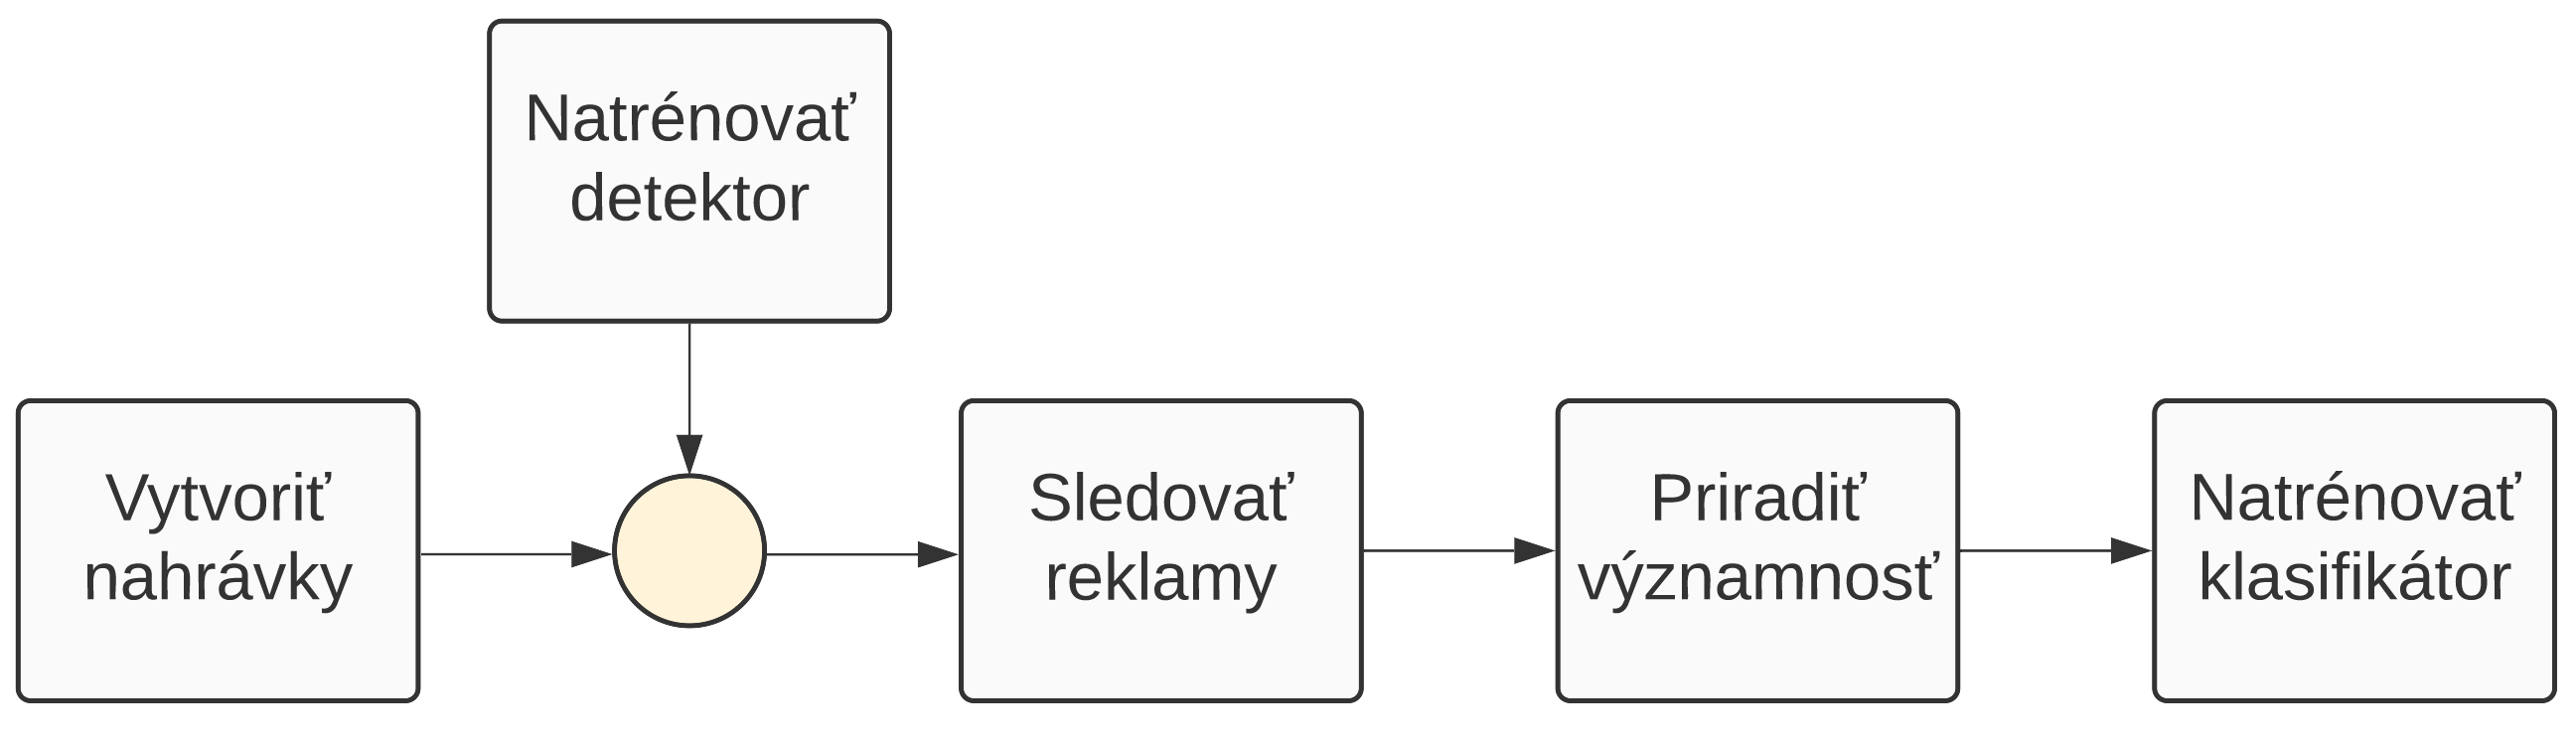
\includegraphics[width=1\textwidth]{images/02/roadmap.png}
%     \caption{Zhrnutý postup navrhnutého riešenia.}
%     \label{img:plan}
% \end{figure}
